\chapter{ELMy H-mode simulations}\label{sec:results}\thispagestyle{fancy}
%%
\begin{wrapfigure}{r}{2cm}
\vspace{-0.5cm}
\includegraphics[width=2cm]{../matlab/pics/40080.eps}
\vspace{-0.5cm}
\end{wrapfigure}
%%
The input data for our simulations were taken from TCV shot \#\Shot\ at time $t = \tZero s$. This choice was made upon many characteristics, mainly that it is a divertor ELMy H-mode with constant ECH power input. Another characteristic is that there is available data from the CXRS diagnostic, which is not yet standard in TCV. On the right we have a poloidal section of the plasma flux surfaces (\#\Shot, $t = \tZero s$).

Simulations have been done for several cases. The reference case is using the self-made $\chi_e$ scaled for the total and pedestal energy, computing the pedestal density using the $L_n \simeq 2 L_T$ scaling except during ELMs. The central density computation uses $V_n / D_n = 1$ to be not too far from the experimental data. This value is well in the range of $[1\ 1.4]$ discussed above. The ion temperature was taken from experimental CXRS data.
%%%%%%%%%% SECTION %%%%%%%%%% {{{1 H-mode simulations
\section{H-mode simulations}\label{sec:results:Hmode}
%%
%%%%%%% SUB %%%%%%% {{{2 Experimental data vs simulation
\subsection{Experimental data vs simulation}\label{sec:results:Hmode:expVSsim}
%%
Running simulations cannot be performed without a special care of what we are doing. Here we compare the electron temperature and density because of their important role and the assurance that the experimental data are very good. The ion temperature is also presented on fig. \ref{fig:results:Hmode:expVSsim:nodesVSsim}. The dots represent the measured data, while the lines are the fitted profiles with upper and lower error boundaries, and the ASTRA output data.

We note that the simulated electron temperature is pretty good matching the experimental data except in the very center. The pedestal density is also well matching, giving us good confidence in the $L_n \simeq 2 L_T$ scaling. We adjusted it to have the best matching achievable, and this gives the relation $L_n \simeq 1.7 L_T$, which is $\nabla n_e / n_e \simeq 0.6\ \nabla T_e / T_e$. Although it was adjusted, this scaling seems to give pretty good results. But the core density appears to be overestimated in the simulation, like the center temperature. This may be due to a sawtooth crash right before the measurements were taken, implying the experimental profiles are post-sawtooth ones.

The $\chi_e$ used in this simulation had been scaled with regards to the total \eqref{eq:confinement:transport:tauE} and pedestal energy \eqref{eq:confinement:Hmode:divertor:WcoreWped}. Figure \ref{fig:results:Hmode:expVSsim:nodesVSsim:chie} shows us that the self-made $\chi_e$ was very different from the one in TCV data nodes, whatsoever its profile or its amplitude.

The ion temperature showed on figure \ref{fig:results:Hmode:expVSsim:nodesVSsim:Ti} is not matching the initial condition showed here as the fitted profile, but is still everywhere in an acceptable range. The boundary condition (at $\rho = 1$) is well in the experimental data.
\begin{figure}[!t]
\begin{center}
\subfloat[\footnotesize Electron temperature.]{\includegraphics[width=5.3cm]{../matlab/pics/40080_0.8_te_equil.eps}\label{fig:results:Hmode:expVSsim:nodesVSsim:Te}}
\hspace{3mm}
\subfloat[\footnotesize Electron density.]{\includegraphics[width=5.3cm]{../matlab/pics/40080_0.8_ne_equil.eps}\label{fig:results:Hmode:expVSsim:nodesVSsim:ne}}
\hspace{3mm}
\subfloat[\footnotesize Ion temperature.]{\includegraphics[width=5.3cm]{../matlab/pics/40080_0.8_ti_nodesVSsim.eps}\label{fig:results:Hmode:expVSsim:nodesVSsim:Ti}}\\
\subfloat[\footnotesize Temperature gradient length.]{\includegraphics[width=5.3cm]{../matlab/pics/40080_0.8_lte_equil.eps}\label{fig:results:Hmode:expVSsim:nodesVSsim:LTe}}
\hspace{3mm}
\subfloat[\footnotesize Density gradient length.]{\includegraphics[width=5.3cm]{../matlab/pics/40080_0.8_lne_equil.eps}\label{fig:results:Hmode:expVSsim:nodesVSsim:Lne}}
\hspace{3mm}
\subfloat[\footnotesize Electron thermal diffusion coefficient.]{\includegraphics[width=5.3cm]{../matlab/pics/40080_0.8_chie_nodesVSsim.eps}\label{fig:results:Hmode:expVSsim:nodesVSsim:chie}}
\end{center}
\vspace{-0.7cm}
\caption{\footnotesize Electron temperature and density with their gradient length, ion temperature and electron thermal diffusivity. The solid blue lines are the simulation output data, while dashed red ones are the experimental data. The ion temperature is presented as function of $\rho_{\psi}$. The electron thermal diffusivity dashed line (linked to the right axis) represents the data computed with the L-mode scripts. (Colors in the electronic version.)\label{fig:results:Hmode:expVSsim:nodesVSsim}}
\vspace{-0.5cm}
\end{figure}
%% }}}2
%%%%%%% SUB %%%%%%% {{{2 Effect of edge EC Heating
\subsection{Effect of edge EC Heating}\label{sec:results:Hmode:edgeECH}
%%
We have altered the ECH profile such that we have only ECH power deposited in the center, but the volume integrated power is the same. We keep the same $\chi_e$ to ease the comparison of the data. The altered ECH profile is shown in \figref{results:Hmode:edgeECH:X3only_equil:ECH} together with the standard case. The energy confinement time being better in the center, it is normal to observe a higher temperature in the center when it is more heated, as we can see in \figref{results:Hmode:edgeECH:X3only_equil:te}. The edge is heated the same, but in this case the heating comes more from the transport. The center density provides high transport of energy through the species, yielding the higher ion temperature shown on \figref{results:Hmode:edgeECH:X3only_equil:ti}.

%What can be noted is a tiny change in the pedestal pressure. The one from this case seems a little lower than that of the reference case. It is also slightly noticeable in the pressure gradient profile. This may be due to the high peaking of the profiles, the low-edge heating implying a slight decrease in the temperature profile.

The electron heat flux (fig.~\ref{fig:results:Hmode:edgeECH:X3only_equil:qe}) shows a clear difference in the core plasma. The pedestal is also affected by this change, but the difference becomes smaller compared to that of the core and both profiles are essentially the same in this edge region. The figure~\ref{fig:results:Hmode:edgeECH:X3only_equil:maxGradPe} shows the pressure gradient to view the position of the maximum, which is the same in both cases.

The ELM cycle will be studied in the next section. Since the changes in the pedestal pressure are not significant, we will shift the time traces to match the initial values of the reference case, in order to facilitate the comparison between these two cases.

\begin{figure}[H]
\begin{center}
\subfloat[\footnotesize Electron temperature.]{\includegraphics[width=5.3cm]{../matlab/pics/40080_0.8_te_equil_X3only.eps}\label{fig:results:Hmode:edgeECH:X3only_equil:te}}
\hspace{3mm}
\subfloat[\footnotesize Ion temperature.]{\includegraphics[width=5.3cm]{../matlab/pics/40080_0.8_ti_equil_X3only.eps}\label{fig:results:Hmode:edgeECH:X3only_equil:ti}}
\hspace{3mm}
\subfloat[\footnotesize Electron density.]{\includegraphics[width=5.3cm]{../matlab/pics/40080_0.8_ne_equil_X3only.eps}\label{fig:results:Hmode:edgeECH:X3only_equil:ne}}\\
\subfloat[\footnotesize ECH deposition profile.]{\includegraphics[width=5.3cm]{../matlab/pics/40080_0.8_ecrh_equil_X3only.eps}\label{fig:results:Hmode:edgeECH:X3only_equil:ECH}}
\hspace{3mm}
%\subfloat[\footnotesize Electron pressure profile.]{\includegraphics[width=5.3cm]{../matlab/pics/40080_0.8_p_e_equil_X3only.eps}\label{fig:results:Hmode:edgeECH:X3only_equil:p_e}}
%\hspace{3mm}
\subfloat[\footnotesize Pressure gradient.]{\includegraphics[width=5.3cm]{../matlab/pics/40080_0.8_maxGradPe_X3only.eps}\label{fig:results:Hmode:edgeECH:X3only_equil:maxGradPe}}
\hspace{3mm}
\subfloat[\footnotesize Electron heat flux.]{\includegraphics[width=5.3cm]{../matlab/pics/40080_0.8_qe_equil_X3only.eps}\label{fig:results:Hmode:edgeECH:X3only_equil:qe}}
\vspace{-0.5cm}
\end{center}
\caption{\footnotesize The electron temperature, density and heat flux, the ion temperature, the pressure gradient and the ECH deposition profiles are shown here to compare the central ECH case to the reference one. The latter is represented by the solid blue line while the dashed red shows the former.\label{fig:results:Hmode:edgeECH:X3only_equil}}
\vspace{-0.5cm}
\end{figure}
%% }}}2
%% }}}1
%%%%%%%%%% SECTION %%%%%%%%%% {{{1 ELMs simulations
\newpage
\section{ELMs simulations}\label{sec:results:ELMs}
%%
%%%%%%% SUB %%%%%%% {{{2 Simulated ELM cycle
\subsection{Simulated ELM cycle}\label{sec:results:ELMs:cycle}
%%
\begin{AllFigs}{stdNoST}{!t}{}{te,ne,lte,lne}{n}{rhosOKplot}{Profiles of the main quantities with the chosen values of $\rho_V$. The vertical dotted lines are the position which will be studied in the time traces.}
\end{AllFigs}
%%
The figure~\AllProfsRef{stdNoST} displays a chosen set of profiles during an ELM cycle together with the chosen values of $\rho_V$ (vertical dotted lines) that will be used to investigate the time traces of the quantities. The left one is the top of the density pedestal, and the other one is at the maximum of the pressure gradient in the equilibrium case. They will respectively be denoted $\rho_1$ and $\rho_2$. The latter happens to be also the surface of $q = 2$. The times are defined according to what we said before (\paref{sim:ELM}), $t = 0$ is the ELM onset, the ELM has a duration of $0.1ms$ and a period of $20ms$.

\begin{AllFigs}{stdNoST}{!t}{}{p_e,ti,itot,ibs}{y}{rhosOKplot}{Profiles of the main quantities with the chosen values of $\rho_V$. The vertical dotted lines are the position which will be studied in the time traces.}
\end{AllFigs}
%%
First looking at the temperature on figure~\AllProfsRef{stdNoST:te}, we note that it recovers pretty fast. The first time is similar to the last one right before the next ELM. The third is $100 \mu s$ after the ELM end and shows that the temperature pedestal has already begun to rebuild itself. But this little start does not give yet $1 / L_{T_e}$ pedestal values as high as pre-crash (fig~\AllProfsRef{stdNoST:lte}). The pedestal density being computed from it (fig.~\AllProfsRef{stdNoST:ne}), we understand that it is not sufficient for the pedestal density to grow. On the density graph we even observe that the density continues to decrease in the pedestal for more than a half millisecond after the ELM stops. We also note that the temperature characteristic length has higher values at the edge of the ELM until $1ms$ after the ELM. This leads to the same remark for the $1 / L_{n_e}$ profile which uses the latter, implying a soft slope for the edge density for a longer time.

Looking closely at the density profiles, we note that at the top of pedestal we also see this phenomenon. This is due to the computation of the density. The ELM makes an almost flat density profile at the edge and a very sharp gradient to match the almost unaffected core density profile. Once the ELM is gone, the normal parameters are applied again and our model tries to make $\nabla n_e / n_e = V_n / D_n$. The inner part has a very low value (see fig. \AllProfsRef{stdNoST:lne}) and therefore tries to reduce the gradient. The pedestal part depends on the $\nabla T_e / T_e$ ratio, which is pretty high at this location right after the crash. Thus we understand that our model tries to flatten the inner density profile while it sharpens the pedestal one.

We used the relation $V_n / D_n \simeq 0.6\ \nabla T_e / T_e$ and we have approximately in the pedestal $L_T \simeq 1.7 L_n$ on figures~\AllProfsRef{stdNoST:lte} and \AllProfsSub{stdNoST:lne}.

\begin{AllFigs}{stdNoST}{!t}{}{q,shear,upl}{y}{rhosOKplot}{Profiles of the main quantities with the chosen values of $\rho_V$. The vertical dotted lines are the position which will be studied in the time traces.}
\end{AllFigs}
%%
Comparing the electron temperature to the ion one on figure~\AllProfsRef{stdNoST:ti}, we note that the latter does not rebuild its pedestal as fast as that of the electron. This is due to the fact that our boundary value for the ion temperature is higher than that of the electrons. Hence when the pedestal flattens for these quantities to the boundary value, the ion temperature becomes higher than the electron one, reversing the sign of the equipartition term. The latter yields a sink for the ions and a source for the electrons. This explains the small decrease observed on the pedestal ion temperature right after the ELM.

Assuming that we have never $T_i > T_e$ in TCV, this reversal of the equipartition is not expected. To prevent this, the ion temperature could be implemented in another way. \cite{andreas2010}~reported that in TCV SN H-mode, we have $T_i \simeq T_e$ for $\rho_{\psi} > 0.85$. It could be interesting to study a case with both boundary temperatures equal $T_{i,a} = T_{e,a}$ and building an ion temperature pedestal on $\chi_i$.

Considering the total and bootstrap current density (figs.~\AllProfsRef{stdNoST:itot} and \AllProfsSub{stdNoST:ibs}), and the loop voltage (\AllProfsRef{stdNoST:upl}), we note that the recovery is pretty fast. For the loop voltage and the total current, around $2ms$ after the crash we have almost completely recovered. The bootstrap current is a little longer because it needs the pressure gradient which depends upon both the temperature and the density. The latter is somehow slower to rebuild its pedestal and therefore slows down the bootstrap recovery.

\begin{AllFigs}{}{!t}{}{te,ne,LTe,Lne}{n}{resultsplotO}{Standard simulated ELM cycle. The solid blue one is at the top of the density pedestal and the dashed red one is at the maximum of $\nabla p$ from equilibrium. Exceptionally shown is the temperature time trace at its top of pedestal on the temperature and temperature gradient length time traces in dash-dotted black.}
\end{AllFigs}
%%
The safety factor profile (figure~\AllProfsRef{stdNoST:q}) is almost constant in time. On the contrary, the magnetic shear (fig.~\AllProfsRef{stdNoST:shear}) shows a clear crash and a recovery time of the same order of the total current density. This means that the flux surfaces are almost unaffected by the ELM according to our model, but the magnetic shear is much more perturbed.

Computing the energy difference, we obtain the proportion of the energy expelled by the ELM. In this reference case, we have $\Delta W / W \simeq 12\%$, which is reasonable for type-I ELMs \cite{andreas2010}, but a little far from the experimental results ($\sim 20\%$). The absolute loss of energy is around $1.8 kJ$.

What can be noted about these profiles is an interesting result in the electron temperature and density (figs.~\AllProfsRef{stdNoST:te} and \AllProfsSub{stdNoST:ne}). The crash lets the center values almost unaffected. Nevertheless, \cite{andreas2010} reported that the ELMs significantly affect the center temperature almost instantaneously. This could lead us to some global confinement phenomena that might happen during the ELM. Another explanation could be with the strong gradient observed on these figures. The ballooning-kink stability criteria are related to the pressure gradient. At the ELM onset, both profiles reveal sharp slopes at the border between the ELM affected zone and the unaffected core. It is thus possible that these gradients then active another ``ELM'' there, and this phenomenon could repeat until it reaches the center. A last explanation we can provide here is that the MHD mode itself could be global.

\begin{AllFigs}{}{!t}{}{p_e,ti,jbs,ibsped,jtot,q}{y}{resultsplotO}{Standard simulated ELM cycle. The quantity ``ibsped'' is the bootstrap current density integrated over the pedestal. The solid blue one is at the top of the density pedestal and the dashed red one is at the maximum of $\nabla p$ from equilibrium.}
\end{AllFigs}
%%
Now we have studied the whole profiles, we can investigate the time traces at the selected locations. The temperature (fig.~\AllFigsRefO{:te}) shows different behavior whether we are looking at the edge of the pedestal or at where we find the maximum pressure gradient in equilibrium. The latter exhibits a shorter characteristic recovery time (about half). However, the former might not show a local confinement time as the global effects can rapidly acts at this position in the temperature core.

The temperature drop at the top of its pedestal is of the order of $0.6 keV$. Experiments reveal that this drop should be around $0.2 keV$ (fig.~6.3 in \cite{andreas2010}), thus it is too high in our simulations.

These time traces exhibit a very fast recovery for the temperature after the crash, which is the observed behavior for type-I ELMs at TCV \cite{andreas2010}. Though, the experimental data show a recovery to the steady-state value less than our simulations ($\sim 300\mu s$ from fig.~6.3 in \cite{andreas2010} instead of $\sim 3ms$ which corresponds to $90\%$ of recovery in fig.~\AllFigsRefO{:te} in the present work). To meet the experimental data, the heat conductivity in the ELM phase may be too much increased in the pedestal (or the pedestal duration may be too long) while in the post-ELM phase it might not be large enough, also in the core region.

\begin{AllFigs}{}{!t}{}{shear,upl}{y}{resultsplotO}{Standard simulated ELM cycle. The solid blue one is at the top of the density pedestal and the dashed red one is at the maximum of $\nabla p$ from equilibrium.}
\end{AllFigs}
%%
Considering the density (fig.~\AllFigsRefO{:ne}), we note that at the top of pedestal, we see the small relaxation we discussed above and will not be discussed here. In the inner part, we see a larger drop, but it occurs \emph{after} the crash. The latter causes only the tiny change we see on the very left of the graph. The following drop is caused by the energy loss, the plasma tries to refill its pedestal after the ELM. Thus here we cannot speak of a recovery time.
		
Comparing with experimental results from \cite{andreas2010} figure~6.4, we note that our pedestal density drop at its top is about $0.6 \cdot 10^{19} m^{-3}$, a little less than what was experimentally observed ($\sim 1 \cdot 10^{19} m^{-3}$). We also have a longer recovery time ($\sim 10ms$) whereas observations of experiments reveal a very fast recovery ($\sim 1ms$) for the density pedestal \cite{andreas2010}. On the other hand, comparison between the temperature and the density shows that the temperature is faster to recover than the density, as is the case in the experimental results.

The temperature (fig.~\AllFigsRefO{:te}), the density (\AllFigsSubO{ne}) and the pressure (\AllFigsSubO{p_e}) time traces reveal that the pressure recovery is more similar to that of the density than that of the temperature and is therefore dominated by the density, in agreement with the experimental observation \cite{andreas2010} figure~6.5. The pressure gradient depends strongly on the density gradient, which we have seen is slower to rebuild than the temperature gradient.
		
Looking closely at the total current density (fig.~\AllFigsRefO{:jtot}), the solid time trace goes down and right after up. This phenomenon happening during the ELM, it will not be discussed here as it is beyond the scope of this work.

We also note that there is a change at about $4ms$ on the time trace of the total current (fig.~\AllFigsRefO{:jtot}) and of the magnetic shear (fig.~\AllFigsRefO{:shear}) at the maximum pressure gradient. This is due to the pedestal building. Indeed, the ELM flattens both temperature and density pedestals. When the relaxation begins, the plasma wants to recover it, implying a sharp increase in the temperature and density gradients. When they come to the desired profile, the gradients decrease. But they decrease too much and have to increase a little again. This strongly affects the pressure.

\begin{figure}[!t]
\begin{center}
\includegraphics[height=8cm,width=12cm]{../matlab/pics/40080_0.8_jalpha_stdNoST.eps}
\vspace{-0.5cm}
\end{center}
\caption{\footnotesize $j - \alpha$ diagram for the reference ELM cycle. Dotted lines are during the ELM crash $0 \le t <0.1$, dash-dotted is for $0.1 \le t < 0.5$, solid lines are $0.5 \le t < 1$ and dashed lines are from 1 to the next ELM (20) with the time in $ms$. $\rho_V = 0.75$ is the top of the density pedestal, $\rho_V = 0.79$ is where this diagram is the largest, $\rho_V = 0.81$ is the top of the temperature pedestal and $\rho_V = 0.86$ is the maximum of the pressure gradient.\label{fig:results:ELM:std:jalpha}}
\vspace{-0.5cm}
\end{figure}
%%
The $j - \alpha$ diagram (fig.~\ref{fig:results:ELM:std:jalpha}) gives information about the MHD instabilities we spoke earlier (\paref{MHD:instab}). Here the cycle is pretty fast to recover its equilibrium state. It is almost finished after only $1ms$. It means that the instability criteria defined in the theory preamble could not, within the model of ELM we used, trigger these instabilities. Though, we discussed of the possibility that the ELM affects the whole plasma. In such a case, the trajectory of $j - \alpha$ may be different and thus could be changing in the last phase before the next ELM.
%%
%% }}}2
%%%%%%% SUB %%%%%%% {{{2 Edge EC heating replaced by central
\newpage
\subsection{Edge EC heating replaced by central}\label{sec:results:ELMs:recover:X3only}
%%
\begin{AllFigs}{X3onlyNoST}{!t}{}{p_e,gradp}{n}{resultsplot}{Comparison between experimental profile and only central ECH. The solid blue line is the standard case, the dashed red one is the central ECH one.}
\end{AllFigs}

We are interested in the way the edge EC heating modifies the dynamic behavior of the plasma. As discussed about the equilibrium profiles, this case presents higher center temperatures. Except for this difference, the profiles are almost similar to that of the reference case and are therefore in appendix \ref{sec:app:graphs:recovery:X3only}.

The time traces at the top of the density pedestal show no significant changes from the reference case (shown in appendix \ref{sec:app:graphs:recovery:X3only}, p. \pageref{sec:app:graphs:recovery:X3only}). We note that they almost all start with a different value, but the slopes are quite the same and the characteristic times do not really vary.

At the maximum pressure gradient, we are interested in the recovery of the pressure gradient. Figure~\AllFigsRef{X3onlyNoST:ped:p_e} shows that the pressure is a little lower in this case as we already saw it. We note that both drop down to the same value and start to recover with the same slope. However, while increasing, the slope of the considered case seems to decrease, yielding no significant improvement in the pressure gradient recovery. If we look at the latter (fig.~\AllFigsRef{X3onlyNoST:ped:gradp}), we find that it has gotten back at $90\%$ of its previous value approximately at the same time as the reference case. The first recovery phase of the pressure gradient lasts about $1.5ms$ as is clearly shown for both cases. This is in good agreement with experimental observations (fig.~6.5 in \cite{andreas2010}).

Other quantities exhibit neither significant modification compared to our reference case.
%%
%There is at least one significant change when replacing edge EC heating by central ECH: the ELM energy expulsion. In this case it is around $\Delta W / W \simeq 10\%$, which is better than in the reference case ($12\%$). This is mainly because we have more energy in the plasma (temperature profile more peaked), here we have about $14\%$ more energy.

\begin{figure}[!t]
\begin{center}
\includegraphics[height=8cm,width=12cm]{../matlab/pics/40080_0.8_jalpha_X3onlyNoST.eps}
\vspace{-0.5cm}
\end{center}
\caption{\footnotesize $j - \alpha$ diagram for the ELM cycle with only central EC heating. Dotted lines are during the ELM crash $0 \le t <0.1$, dash-dotted is for $0.1 \le t < 0.5$, solid lines are $0.5 \le t < 1$ and dashed lines are from 1 to the next ELM (20) with the time in $ms$. $\rho_V = 0.75$ is the top of the density pedestal, $\rho_V = 0.79$ is where this diagram is the largest, $\rho_V = 0.81$ is the top of the temperature pedestal and $\rho_V = 0.86$ is the maximum of the pressure gradient.\label{fig:results:ELM:X3only:jalpha}}
\vspace{-0.5cm}
\end{figure}
%%
Looking at the $j - \alpha$ diagram (\figref{results:ELM:X3only:jalpha}), we note no significant change in the aspect compared to the reference case (\figref{results:ELM:std:jalpha}). The one from this case seems a little shifted downwards. This is because the center current density is higher, due to the higher central temperature, which decreases the normalized edge current density.
%% }}}2
%%%%%%% SUB %%%%%%% {{{2 Varying $D_n$
\subsection{Varying $D_n$}\label{sec:results:ELMs:recover:Dn}
%%
\begin{figure}[!b]
\begin{center}
\includegraphics[width=7cm]{../matlab/pics/40080_0.8_ne_rhosOK_Dn01NoST.eps}
\vspace{-7mm}
\end{center}
\caption{\footnotesize Profiles of the main quantities for an inter-ELM with particle diffusivity divided by ten.\label{fig:results:ELMs:rhosOK:Dn01NoST:ne}}
%\vspace{-5mm}
\end{figure}
%%
When varying the particle diffusion coefficient, we therefore change the dynamical behavior of the particles. Recalling of the definition of the diffusion time \eqref{eq:confinement:transport:taus:taun}, it will have a strong effect on it and therefore slow down or speed up the density processes. The cases considered here are ``Dn01'', ``Dn05'' and ``Dn10'' where we have respectively divided by ten, by two and multiplied by ten the particle diffusion coefficient in the inter-ELM period, and the pinch velocity as well to keep the same ratio $V_n / D_n$. The equilibrium profiles being unchanged, the profiles of these case do not exhibit a lot of difference comparing to the reference case. We are only showing here the density profiles for the ``Dn01'' case, the other profiles and cases' profiles being in appendix \ref{sec:app:graphs:recovery:Dn} (p.~\pageref{sec:app:graphs:recovery:Dn}).

\begin{AllFigs}{DnNoST}{!t}{}{te,ne,p_e}{n}{resultsplot}{Comparison between different values for Dn. The solid blue line is the reference case, the dashed red one is the ``Dn10'' case, the dash-dotted dark green is ``Dn05'' and the dotted black is ``Dn01''.}
\end{AllFigs}
%%
The density profile (fig.~\AllProfsRef{Dn01NoST:ne}) shows that the density pedestal has been much more flattened among the ELMs than the reference case (fig.~\AllProfsRef{stdNoST:ne}), and the central density has increased compared to the latter.% For further analysis, we will shift the traces for them to match the initial values.

\begin{AllFigs}{DnNoST}{!t}{}{LTe,Lne,ti}{y}{resultsplot}{Comparison between different values for Dn. The solid blue line is the reference case, the dashed red one is the ``Dn10'' case, the dash-dotted dark green is ``Dn05'' and the dotted black is ``Dn01''.}
\end{AllFigs}
%%
The time traces (fig.~\ref{fig:results:ELMs:DnNoST}), particularly the density time traces, exhibit a clear difference when varying $D_n$. We understand that lower diffusivity yields a slower behavior for the density. This has an impact on the other quantities too since they depend on the density. For the lowest particle diffusivity (``Dn01''), we observe that this case has a decreasing temperature at the end of the cycle, before the next crash. This might be due to the slow recovery of the density: the crash decreased the temperature and the density, the former rebuilding right after, faster than the latter. This means that the heating is well spread among the plasma very fast compared to the change in density, having a near-equilibrium temperature profile. But the density continues to regrow and soon the heating losses become more important than the source and the temperature decreases. The ion temperature is also affected by this change since the source of ion heating is the equipartition depending on the collisionality and on the electron temperature. We observe this for all but the high-diffusivity case after around $10ms$.

These changes are less visible at the maximum of the pressure gradient, because here the temperatures are also flattened by the crash.

Looking at the total current density and the shear time traces (figs.~\AllFigsRef{DnNoST:core:jtot}, \AllFigsSub{DnNoST:ped:jtot}, \AllFigsSub{DnNoST:core:shear} and \AllFigsSub{DnNoST:ped:shear}), we note that at about $5ms$ we seem to have a change in the behavior of these quantities. In the other cases this change is also present but comes faster and has already been discussed. This is particularly visible at the maximum of the pressure gradient.

%Almost all these time traces show that the cases ``Dn05'' and ``Dn10'' seem to be opposite as compared to the reference case. This might be due to the recovery dependence on $D_n$ that may be not linear or this may be caused by the different initial conditions.
%%
Increasing the density recovery time means it would not necessarily have finished to recover when the next ELM comes. We understand that stopping the recovery earlier will prevent the density to recover as much as it was pre-crash, yielding a gradual decrease.

The energy loss for the tenth-diffusivity case is not quite the same as the reference case. Indeed, it has decreased to $9\%$ (approximately $1.5 kJ$). This is explained by the increase of the temperature that compensate the loss of density from the energy point of view. The total energy is almost the same, but the density has been considerably decreased at the considered ELM. Our ELM model is set to not flatten completely the density pedestal. Since the latter did not fully recover, it is already a bit flat, hence the ELM cannot decrease it much.

The $j - \alpha$ diagram for the tenth-diffusivity case (\figref{results:ELM:Dn01:jalpha}) seems a little changed compared to (\figref{results:ELM:std:jalpha}). We note that the pressure gradient seems lower, due to the progressive flattening of the density pedestal, but we also note that the cycles seems more compact. This is due to the density recovery time that has been multiplied by ten. The pressure gradient and the edge current density are also affected by this change, particularly visible in the fourth phase (dashed lines).

\begin{AllFigs}{DnNoST}{H}{}{jtot,jbs,ibsped}{y}{resultsplot}{Comparison between different values for Dn. The solid blue line is the reference case, the dashed red one is the ``Dn10'' case, the dash-dotted dark green is ``Dn05'' and the dotted black is ``Dn01''.}
\end{AllFigs}
%%
\begin{AllFigs}{DnNoST}{H}{}{shear,upl}{y}{resultsplot}{Comparison between different values for Dn. The solid blue line is the reference case, the dashed red one is the ``Dn10'' case, the dash-dotted dark green is ``Dn05'' and the dotted black is ``Dn01''.}
\end{AllFigs}
%%
\begin{figure}[H]
\vspace{-6mm}
\begin{center}
\includegraphics[height=8cm,width=12cm]{../matlab/pics/40080_0.8_jalpha_Dn01NoST.eps}
\vspace{-5mm}
\end{center}
\caption{\footnotesize $j - \alpha$ diagram for the ELM cycle of ``Dn01''. Dotted lines are during the ELM crash $0 \le t < 0.1$, dash-dotted is for $0.1 \le t < 0.5$, solid lines are $0.5 \le t < 1$ and dashed lines are from 1 to the next ELM (20) with the $t$ in $ms$. $\rho_V = 0.75$ is the top of the density pedestal, $\rho_V = 0.79$ is where this diagram is the largest, $\rho_V = 0.81$ is the top of the temperature pedestal and $\rho_V = 0.86$ is the maximum of the pressure gradient.\label{fig:results:ELM:Dn01:jalpha}}
\vspace{-5mm}
\end{figure}
%%
%% }}}2
%%%%%%% SUB %%%%%%% {{{2 First ELM
\subsection{First ELM}\label{sec:results:ELMs:recover:first}
%%
We can now wonder if the first ELM is the same as the following ones or if we have a behavior such that ELMs do not allow to recover fully the steady-state profiles. To investigate this we will compare the first ELM to that previously studied, say the eleventh. This is done for the different cases where we have changed $D_n$.

%%% STD %%%
\begin{AllFigs}{stdNoSTfirst}{!t}{}{ne}{n}{resultsplot}{Comparison between first and non-first ELM. The solid blue line is the non-first from the reference case while the dashed red one is the first.}
\end{AllFigs}
%%
The standard case show no significant change between the first and the non-first ELMs. The most significant one is on the density time trace at the top of its pedestal (fig.~\AllFigsRef{stdNoSTfirst:core:ne}). We note that the non-first recovers to the pre-crash value just before the next crash, whether the first suffers some losses.

\begin{figure}[!t]
\begin{center}
\vspace{1mm}
\includegraphics[height=8cm,width=12cm]{../matlab/pics/40080_0.8_jalpha_stdNoSTfirst.eps}
\vspace{-5mm}
\end{center}
\caption{\footnotesize $j - \alpha$ diagram for the first ELM cycle of the reference case. Dotted lines are during the ELM crash $0 \le t <0.1$, dash-dotted is for $0.1 \le t < 0.5$, solid lines are $0.5 \le t < 1$ and dashed lines are from 1 to the next ELM (20) with the time in $ms$. $\rho_V = 0.75$ is the top of the density pedestal, $\rho_V = 0.79$ is where this diagram is the largest, $\rho_V = 0.81$ is the top of the temperature pedestal and $\rho_V = 0.86$ is the maximum of the pressure gradient.\label{fig:results:ELM:first:jalpha}}
\vspace{-0.5cm}
\end{figure}
%%
Comparing the $j - \alpha$ graph of the first ELM in the reference case (\figref{results:ELM:first:jalpha}) to that of the non-first (\figref{results:ELM:std:jalpha}), we observe that the diagram has been slightly shifted towards the bottom-left corner from the first to the elventh, yielding a gradual decrease of both the pressure gradient and the edge current density among the ELMs.

\begin{AllFigs}{Dn01NoSTfirst}{!t}{}{te,ne,p_e}{n}{resultsplot}{Comparison between first and non-first ELM. The solid blue line is the non-first from the ``Dn01'' case while the dashed red one is the first.}
\end{AllFigs}
%%
%%% Dn10-05 %%%
The case ``Dn10'' shows less of these, but these changes are also present (results shown in appendix \ref{sec:app:graphs:recovery:first}). Comparing the first ELM to the non-first for the case with half-diffusion coefficient, the density recovery time is not much affected. Other quantities show no significant changes. Graphs can be seen in appendix \ref{sec:app:graphs:recovery:first}.

%%% Dn01 %%%
\begin{AllFigs}{Dn01NoSTfirst}{!t}{}{LTe,Lne,ti}{y}{resultsplot}{Comparison between first and non-first ELM. The solid blue line is the non-first from the ``Dn01'' case while the dashed red one is the first.}
\end{AllFigs}
%%
The tenth-diffusivity case is more interesting (fig.~\AllFigsRef{Dn01NoSTfirst}). If we recall of the diffusion time definition \eqref{eq:confinement:transport:taus:taun}, dividing the particle diffusivity by ten means multiplying the diffusion time by the same factor. It is then understandable that the recovery time, which is related to the diffusion time, is longer and that the recovery may not be finished when the next ELM comes. This yields a gradual decrease.

\begin{AllFigs}{Dn01NoSTfirst}{!t}{}{jtot,jbs,q}{y}{resultsplot}{Comparison between first and non-first ELM. The solid blue line is the non-first from the ``Dn01'' case while the dashed red one is the first.}
\end{AllFigs}
%%
We clearly see that this change affects a lot the plasma. The density time traces (figures~\AllFigsRef{Dn01NoSTfirst:core:ne} and \AllFigsSub{Dn01NoSTfirst:ped:ne}) show that its pedestal does not fully recover when the first happens, and almost recovers for the non-first but not fully. The first presents a very large drop of density at the top of its pedestal; but this drop does not come from the ELM itself as it happens during the recovery phase. The ELM losses there are of the same order as the non-first. At the maximum of the pressure gradient, on the other hand, the ELM creates a huge loss of particles. Building the pedestal again yield the core has to provide particles too.

\begin{AllFigs}{Dn01NoSTfirst}{!t}{}{shear,upl}{y}{resultsplot}{Comparison between first and non-first ELM. The solid blue line is the non-first from the ``Dn01'' case while the dashed red one is the first.}
\end{AllFigs}
%%
This density difference yields a change in the other way for the temperature since the heating remains the same, increasing the core temperature as can be seen in fig.~\AllFigsRef{Dn01NoSTfirst:core:te}. This loss also means less equipartition which reduces the ion temperature as shown in figures~\AllFigsRef{Dn01NoSTfirst:core:ti} and \AllFigsSub{Dn01NoSTfirst:ped:ti}. The safety factor (shown in figures~\AllFigsRef{Dn01NoSTfirst:core:q} and \AllFigsSub{Dn01NoSTfirst:ped:q}) also exhibits a more pronounced behavior in this case.
%% }}}2
%%%%%%% SUB %%%%%%% {{{2 Link between $D_n$ and the ELM period
\subsection{Link between $D_n$ and the ELM period}\label{sec:results:ELMs:recover:delta}
%%
\begin{AllFigs}{DnVSdeltaNoST}{!t}{}{ne}{n}{resultsplot}{Density comparison between for different particle diffusion coefficients and different inter-ELM periods. The solid blue line is the reference case, the dashed red one is the ``Dn05'' case, the dash-dotted dark green is ``Dn01'' and the dotted black is with half the ELM period. The left figure shows the traces at the top of the density pedestal while the right one is at the maximum of the pressure gradient.}
\end{AllFigs}
%%
The density time traces of the reduced particle diffusion coefficients seemed to be stretched and cut after the same time anyway. This looks like we had reduced the ELM period and normalized the abscissa. We try this case by dividing the ELM period by two to compare the change of the particle diffusivity to that of the ELM period. To compare the results, we now display them using the ELM period as abscissa, meaning zero is the crash considered and one is the next crash. We have tested a case with half the period of the reference case. The ELM duration was kept the same to ensure the post-crash values to be accurate, which yields for a normalized abscissa that the case of half-period seems to have an ELM duration of twice those of the other cases.

The density time traces (figures~\AllFigsRef{DnVSdeltaNoST:core:ne} and \AllFigsSub{DnVSdeltaNoST:ped:ne}) show what we expected: the reduction of the ELM period acts in the same way as the reduction of the particle diffusion coefficient. The quantification of this observation is more difficult. We note that dividing the period by two seems to change the plasma like dividing the diffusivity by the same factor. The link between the particle diffusivity and the ELM period is obviously that when reducing one of them, the density has less time to recover, which may lead to a gradual decrease. Further studies are required to establish this link.

The other time traces are shown in appendix \ref{sec:app:graphs:recovery:delta}. We must be careful with this abscissa when speaking of the characteristic times, because it is normalized to the ELM period. As we guessed from the figure~\AllFigsRefO{}, they do not show any significant difference.
%% }}}2
%%%%%%% SUB %%%%%%% {{{2 Varying the ELM interaction range
\subsection{Varying the ELM interaction range}\label{sec:results:ELMs:rho}
%%
Our reference case used an ELM range that was based upon the density pedestal width. This choice was mainly motivated by experimental observations \cite{bruckhart2010}. MHD activity is not necessarily linked to transport activity. Therefore these two widths have no reason to be the same. It is of interest to change the ELM interaction range to observe the behavior of the transport phenomena when the MHD activity range is not linked to them. We have thus run a simulation with the ELM interaction range doubled. The density pedestal has a width of around $3cm$ thus we now take an interaction range of $6cm$ for the ELM (approximately $0.67 < \rho_{\Phi} \le 1$ instead of $0.78 < \rho_{\Phi} \le 1$).

\begin{AllFigs}{width2NoST}{!t}{}{te,ne}{n}{rhosOKplot}{Profiles of the main quantities for the case where we double the ELM range.}
\end{AllFigs}
%%
The profiles of figure~\AllProfsRef{width2NoST} show the same behavior as the reference case (fig.~\AllProfsRef{stdNoST}) except that the range of the ELM is broader.

\begin{AllFigs}{width2NoST}{!t}{}{te,ne,ti}{n}{resultsplot}{Time traces of the main quantities for the case where we double the ELM range.}
\end{AllFigs}
%%
Looking at the time traces, the temperature (fig.~\AllFigsRef{width2NoST:core:te} and \AllFigsSub{width2NoST:ped:te}) has a much larger drop, and the recovery takes much more time than in the standard case. This is because the temperature has crashed on a very broad region (around the third of the plasma radius) and thus the energy has been lost over the latter. It is understandable that it needs more time since it has more energy to recover.

The temperature gradient length also climbs less at $\rho_1$, because the connection between the region flattened by the ELM and the intact region is more inside the plasma. The ion temperature (fig.~\AllFigsRef{width2NoST:core:ti}) has the same behavior as the electron's since its heat source comes from the electron energy.

The density at the top of its pedestal (shown on fig.~\AllFigsRef{width2NoST:core:ne}) also has the relaxation due to our model: right after the crash the temperature gradient becomes high for the recovery, implying a high value for $V_n / D_n$. As the temperature recovers, its gradient flattens, reducing the previous ratio. Since it only changes the pinch velocity ($D_n = 0.2 \chi_E$), it means that the first phase after the crash has a high pinch velocity then lower, allowing particles to move faster at first but slower afterwards. This is what we observe on this time trace.

At $\rho_2$ (figure~\AllFigsRef{width2NoST:ped:ne}) we have the same behavior as the temperature showed at $\rho_1$, a longer recovery time due to the larger losses. Both density gradient length (figs.~\AllFigsRef{width2NoST:core:Lne} and \AllFigsSub{width2NoST:ped:Lne}) also take more time to recover.

These facts imply that the pressure also recovers slower in this case and so does the pedestal bootstrap current. The total current density time traces (figs.~\AllFigsRef{width2NoST:core:jtot} and \AllFigsSub{width2NoST:ped:jtot}) seem shifted due to the ELM shift. The time trace here at $\rho_1$ is somehow like that of the reference case at $\rho_2$.

The safety factor still does not vary much, but at $\rho_2$ we see a larger recovery time which is what we expected since it depends on the currents. The magnetic shear also presents the same behavior as the current densities, more clearly than the safety factor.

The ELM being much larger, we understand that the energy losses here are higher. The absolute energy drop is about $3.2 kJ$, almost twice as much as the reference case. Also, the plasma energy is higher, because the temperature has grown from the gradual decrease of density. The central pre-crash electron temperature is around $0.5 keV$ higher here than in the reference case.

The MHD diagram for this case, \figref{results:ELM:width2:jalpha}, is completely different to that of the reference case (\figref{results:ELM:std:jalpha}). Here we only have the ELM crash making a pressure gradient loss at almost constant edge current density. There is a small loss of edge current density only at the end of the crash.

The presented cycles are all rebuilding the same way on this diagram. First the normalized edge current density decreases, probably due to the loss of pressure gradient. The resistive time $\tau_{\eta}$ \eqref{eq:confinement:transport:taus:taueta} seems to be longer than the energy confinement time \eqref{eq:confinement:transport:tauE}. Then the pressure gradient builds up and finally both increase. Depending on the location, the normalized edge current density increases more or less fast. At the top of the density pedestal $\rho_V = 0.75$, the pressure gradient and the normalized edge current density have already begun to increase after only $0.5ms$, whilst at the maximum of the pressure gradient $\rho_V = 0.86$ only the pressure gradient grows up until $1ms$ before the normalized edge current density begins too.

We note that the pressure gradient grows much more at the maximum of itself than at any other location displayed. Unlike the reference case, we have a longer path for the last phase before the next ELM. The pressure gradient needs much more time to rebuild since the density has been affected further than the top of its pedestal.

\begin{AllFigs}{width2NoST}{H}{}{LTe,Lne,p_e}{y}{resultsplot}{Time traces of the main quantities for the case where we double the ELM range.}
\end{AllFigs}
%%
\begin{AllFigs}{width2NoST}{H}{}{jtot,jbs,ibsped}{y}{resultsplot}{Time traces of the main quantities for the case where we double the ELM range.}
\end{AllFigs}
%%
\begin{AllFigs}{width2NoST}{H}{}{q,shear,upl}{y}{resultsplot}{Time traces of the main quantities for the case where we double the ELM range.}
\end{AllFigs}
%%
\begin{figure}[H]
\begin{center}
\includegraphics[height=8cm,width=12cm]{../matlab/pics/40080_0.8_jalpha_width2NoST.eps}
\vspace{-0.5cm}
\end{center}
\caption{\footnotesize $j - \alpha$ diagram for the wider ELM cycle. Dotted lines are during the ELM crash $0 \le t <0.1$, dash-dotted is for $0.1 \le t < 0.5$, solid lines are $0.5 \le t < 1$ and dashed lines are from 1 to the next ELM (20) with the time in $ms$. $\rho_V = 0.75$ is the top of the density pedestal, $\rho_V = 0.79$ is where this diagram is the largest, $\rho_V = 0.81$ is the top of the temperature pedestal and $\rho_V = 0.86$ is the maximum of the pressure gradient.\label{fig:results:ELM:width2:jalpha}}
\vspace{-0.5cm}
\end{figure}
%%
%% }}}2
%% }}}1
